\chapter{Priprava na 5. laboratorijske vaje}
\section{Minimalne oblike zapisa preklopnih funkcij}

Minimalna oblika zapisa preklopne funkcije podaja najkrajši možen zapis te funkcije. Poznamo več minimalnih oblik zapisa. Pogledali si bomo sledeče:
\begin{itemize}
\item minimalna disjunktivna normalna oblika (MDNO): določa najkrašo disjunktivno normalno obliko zapisa preklopne funkcije,
\item minimalna konjunktivna normalna oblika (MKNO): določa najkrašo konjunktivno normalno obliko zapisa preklopne funkcije,
\item minimalna normalna oblika (MNO): določa nakrajšo normalno obliko zapisa preklopne funkcije.
\end{itemize}

Pri določanju minimalne disjunktivne normalne oblike (MDNO) izhajamo iz iskanja \emph{glavnih vsebovalnikov}. Glavni vsebovalnik predstavlja najkrajši konjunktivni izraz, ki je skupen podmnožici mintermov, ki sestavljajo PDNO podane funkcije. Najmanjša množica glavnih vsebovalnikov, ki skupaj pokrijejo celotno množico mintermov v PDNO, predstavlja minimalno disjunktivno normalno obliko.\\

Pri določanju minimalne konjunktivne normalne oblike (MKNO) izhajamo iz določanja MDNO negirane funkcije, ki jo z uporabo DeMorganovega pravila pripeljemo do konjunktivne oblike.\\

Pri določanju minimalne normalne oblike (MNO) upoštevamo dejstvo, da MNO predstavlja krajšo izmed MDNO in MKNO.\\

Glavne vsebovalnike iščemo na podlagi \emph{sosednosti} med konjunktivni izrazi. Dva konjunktivna izraza sta sosedna, če se razlikujeta po natanko eni negaciji:
\begin{itemize}
\item izraza $x_{1}^{w_1} \cdot x_{2}^{w_2} \cdot ... \cdot x_{i}^{w_i} \cdot ... \cdot x_{n}^{w_n}$ in $x_{1}^{w_1} \cdot x_{2}^{w_2} \cdot ... \cdot x_{i}^{\ol w_i} \cdot ... \cdot x_{n}^{w_n}$ sta sosedna, ker se razlikujeta le po negaciji nad vhodno spremenljivko z indeksom $i$.
\end{itemize}
V splošnem velja, da ima izraz, ki vsebuje $n$ vhodnih spremenljivk, $n$ sosednih izrazov.

\begin{zgled}
Zapiši vse izraze, ki so sosedni izrazu $x_1 \ol x_2 x_4$.\\
\end{zgled}
\begin{resitev}
V sosednih izrazih nastopajo enake spremenljivke kot v izhodiščnem izrazu. Od izhodiščnega izraza se sosedni razlikujejo po natanko eni negaciji. Sosedni izrazi so torej:
\begin{itemize}
\item $\ol x_1 \ol x_2 x_4$,
\item $x_1 x_2 x_4$ in
\item $x_1 \ol x_2 \ol x_4$.
\end{itemize}

\end{resitev}

Glavni vsebovalnik dveh sosednih izrazov določimo z upoštevanjem lastnosti, da je disjunkcija dveh termov, ki se razlikujeta natanko po negaciji nad eno spremenljivko, neodvisna od vrednosti te spremenljivke. Glavni vsebovalnik dveh sosednih izrazov $x_{1}^{w_1} \cdot x_{2}^{w_2} \cdot ... \cdot x_{i-1}^{w_{i-1}} \cdot x_{i}^{w_i} \cdot x_{i+1}^{w_{i+1}} \cdot ... \cdot x_{n}^{w_n}$ in $x_{1}^{w_1} \cdot x_{2}^{w_2} \cdot ... \cdot x_{i-1}^{w_{i-1}} \cdot x_{i}^{\ol w_i} \cdot x_{i+1}^{w_{i+1}} \cdot ... \cdot x_{n}^{w_n}$ je torej izraz $x_{1}^{w_1} \cdot x_{2}^{w_2} \cdot ... \cdot x_{i-1}^{w_{i-1}} \cdot x_{i+1}^{w_{i+1}} \cdot ... \cdot x_{n}^{w_n}$. 

\begin{zgled}
Določi glavni vsebovalnik izrazov $\ol x_1 \ol x_2 \ol x_3 x_4$ in $x_1 \ol x_2 \ol x_3 x_4$.\\
\end{zgled}
\begin{resitev}
Izraza se razlikujeta le po negaciji nad spremenljivko $x_1$. Disjunkcija med izrazoma je torej neodvisna od vrednosti te spremenljivke, zato je njun glavni vsebovalnik $\ol x_2 \ol x_3 x_4$.

\end{resitev}



\section{Veitchev postopek minimizacije}
Veitchev postopek minimizacije izkorišča lastnosti Veitchevega diagrama. Sosednost mintermov je namreč neposredno povezana s sosednostjo celic v diagramu. Pri celicah, ki se nahajajo na robovih diagrama se sosednost prenaša na zrcalno stran (glej sliko \ref{fig:Veitch_sosednost}).

\begin{figure}[ht]
\begin{center}
	\begin{tabular}{ccc}
		
\includegraphics{veitch_sosednost-1.eps} & 
\includegraphics{veitch_sosednost-2.eps} & 
\includegraphics{veitch_sosednost-3.eps}\\
		(a) & (b) & (c)\\
	\end{tabular}		
	\begin{tabular}{cc}
		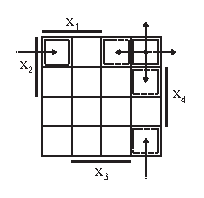
\includegraphics{veitch_sosednost-4.eps} & 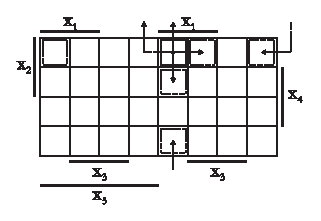
\includegraphics{veitch_sosednost-5.eps}\\
		(d) & (e)\\
	\end{tabular}	
	
\end{center}
\caption{Slika (a) prikazuje sosednost v Veitchevem diagramu za 1 vhodno spremenljivko, slika (b) za 2, slika (c) za 3, slika (d) za 4, slika (e) pa za 5.}
\label{fig:Veitch_sosednost}
\end{figure}

\begin{zgled}
V Veitchevem diagramu za 4 spremenljivke označi izraze, ki so sosednji izrazu $m_{14} \vee m_{15}$.\\
\end{zgled}
\begin{resitev}
Izraz zapišimo v razširjeni obliki: 
$$ m_{14} \vee m_{15} = x_1 x_2 x_3 \ol x_4 \vee x_1 x_2 x_3 x_4 = x_1 x_2 x_3$$

Sosedni izrazi so torej:
\begin{itemize}
\item $\ol x_1 x_2 x_3 = \ol x_1 x_2 x_3 \ol x_4\vee \ol x_1 x_2 x_3 x_4 = m_{6} \vee m_7$ 
\item $x_1 x_2 \ol x_3 = x_1 x_2 \ol x_3 \ol x_4 \vee x_1 x_2 \ol x_3 x_4 = m_{12} \vee m_{13}$
\item $x_1 \ol x_2 x_3 = x_1 \ol x_2 x_3 \ol x_4 \vee x_1 \ol x_2 x_3 x_4= m_{10} \vee m_{11}$ 
\end{itemize}

Veitchev diagram z označemi sosednimi izrazi prikazuje slika \ref{fig:Veitch_sosednost_zgled_4}.

\begin{figure}[ht]
\begin{center}
	
\includegraphics{veitch_sosednost-zgled-4.eps}
\end{center}
\caption{Izrazi, ki so sosedni izrazu $m_{14} \vee m_{15}$.}
\label{fig:Veitch_sosednost_zgled_4}
\end{figure}

\end{resitev}

\begin{zgled}
V Veitchevem diagramu za 5 spremenljivk označi izraze, ki so sosednji izrazu $m_{22} \vee m_{30}$.\\
\end{zgled}
\begin{resitev}
Izraz zapišimo v razširjeni obliki: 
$$ m_{22} \vee m_{30} = x_1 \ol x_2 x_3 x_4 \ol x_5 \vee x_1 x_2 x_3 x_4 \ol x_5 = x_1 x_3 x_4 \ol x_5$$

Sosedni izrazi so torej:
\begin{itemize}
\item $\ol x_1 x_3 x_4 \ol x_5$
\item $x_1 \ol x_3 x_4 \ol x_5$
\item $x_1 x_3 \ol x_4 \ol x_5$
\item $x_1 x_3 x_4 x_5$
\end{itemize}

Veitchev diagram z označemi sosednimi izrazi prikazuje slika \ref{fig:Veitch_sosednost_zgled_5}.

\begin{figure}[ht]
\begin{center}
	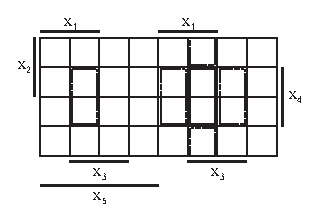
\includegraphics{veitch_sosednost-zgled-5.eps}
\end{center}
\caption{Izrazi, ki so sosedni izrazu $m_{22} \vee m_{30}$.}
\label{fig:Veitch_sosednost_zgled_5}
\end{figure}

\end{resitev}


\subsection{Določanje minimalne normalne oblike z Veitchevim diagramom}

Za minimalno normalno obliko (MNO) velja, da predstavlja krajšo izmed minimalne disjunktivne normalne oblike (MDNO) in minimalne konjunktivne normalne oblike (MKNO). Za določitev MNO moramo torej najprej določiti MDNO in MKNO.

\subsubsection{Določanje minimalne disjunktivne normalne oblike z Veitchevim diagramom}
Postopek določanja je sledeč:
\begin{enumerate}
\item Funkcijo predstavimo z Veitchevim diagramom.
\item Poiščemo glavne vsebovalnike, tako da med seboj združujemo čim večje število sosednih mintermov, pri katerih je funkcijska vrednost enaka 1. Združujemo lahko 1,2,4,8,16,... mintermov. Iščemo najmanjši nabor pokritij, s katerim pokrijemo vse enice. V vsakem koraku poskušamo dobiti čim večje pokritje, saj s tem izločimo večje število vhodnih spremenljivk.
\item Zapišemo MDNO na podlagi glavnih vsebovalnikov.
\end{enumerate}

\subsubsection{Določanje minimalne konjunktivne normalne oblike z Veitchevim diagramom}
\begin{enumerate}
\item Negirano funkcijo predstavimo z Veitchevim diagramom.
\item Poiščemo MDNO negirane funkcije.
\item Negiramo MDNO negirane funkcije, s čimer dobimo izhodiščno funkcijo.
\item Z upoštevanjem DeMorganovega pravila funkcijo prevedemo v MKNO.
\end{enumerate}

\subsubsection{Določanje minimalne normalne oblike}
\begin{enumerate}
\item Določimo število operatorjev (logičnih vrat) in operandov (vhodov) za MDNO in za MKNO posebej. Negacij ne štejemo.
\item Minimalna oblika je tista, ki ima manjše število operatorjev. Če je število operatorjev pri obeh enako, je minimalna tista, ki ima manjše število operandov.
\end{enumerate}

\begin{zgled}
Za funkcijo $f(x_1,x_2,x_3,x_4) = \vee^4(0,4,8,9,10,11,12)$ določi minimalno normalno obliko.\\
\end{zgled}
\begin{resitev}
Najprej določimo MDNO:

\begin{enumerate}
\item Narišemo Veitchev diagram funkcije in označimo glavne vsebovalnike (Slika \ref{fig:Veitch_MDNO}).

\begin{figure}[ht]
\begin{center}
	
\includegraphics{veitch_MDNO.eps}
\end{center}
\caption{Glavni vsebovalniki funkcije $\vee^4(0,4,8,9,10,11,12)$.}
\label{fig:Veitch_MDNO}
\end{figure}

\item Izpišemo glavne vsebovalnike in s tem MDNO:
$$f(x_1,x_2,x_3,x_4)=x_1 \ol x_2 \vee \ol x_3 \ol x_4$$
\end{enumerate}

Potem določimo MKNO:
\begin{enumerate}
\item Narišemo Veitchev diagram negirane funkcije $\ol{f(x_1,x_2,x_3,x_4)}$= \\$\vee^4(1,2,3,5,6,7,13,14,15)$ in označimo glavne vsebovalnike (Slika \ref{fig:Veitch_MKNO}). 
\begin{figure}[ht]
\begin{center}
	\begin{tabular}{cccc}
		
\includegraphics{veitch_MKNO1.eps} & 
\includegraphics{veitch_MKNO2.eps} & 
\includegraphics{veitch_MKNO3.eps} & 
\includegraphics{veitch_MKNO4.eps}\\
		(a) & (b) & (c) & (d)\\
	\end{tabular}		 	
\end{center}
\caption{Glavni vsebovalniki funkcije $\vee^4(1,2,3,5,6,7,13,14,15)$. Slika (a) prikazuje glavni vsebovalnik $\ol x_1 x_3$, slika (b) $x_2 x_3$, slika (c) $\ol x_1 x_4$, slika (d) pa $x_2 x_4$.}
\label{fig:Veitch_MKNO}
\end{figure}

\item Izpišemo glavne vsebovalnike, ki določajo negirano funkcijo: $\ol{f(x_1,x_2,x_3,x_4)} = \ol x_1 x_3 \vee x_2 x_3 \vee \ol x_1 x_4 \vee x_2 x_4$. S tem dobimo MDNO negirane funkcije.
\item Dobljeno MDNO negiramo, uporabimo DeMorganovo pravilo in dobimo MKNO:  $f(x_1,x_2,x_3,x_4) = \ol{\ol x_1 x_3 \vee x_2 x_3 \vee \ol x_1 x_4 \vee x_2 x_4} = (x_1 \vee \ol x_3)(\ol x_2 \vee \ol x_3)(x_1 \vee \ol x_4)(\ol x_2 \vee \ol x_4)$.
\end{enumerate}

Sedaj lahko določimo MNO:
\begin{enumerate}
\item Določimo število operatorjev pri MDNO (za realizacijo potrebujemo dvoja AND vrata in ena OR vrata): $2+1=3$.
\item Določimo število operandov pri MDNO (2 vhoda v prva AND vrata, 2 vhoda v druga AND vrata, 2 vhoda v OR vrata): $2+2+2=6$.
\item Zapišemo par število operatorjev/število operandov za MDNO: $[3,6]$.
\item Določimo število operatorjev pri MKNO (za realizacijo potrebujemo ena AND vrata in štiri OR vrata): $1+4=5$.
\item Določimo število operandov pri MKNO (AND vrata so 4-vhodna, vsa OR vrata pa 2-vhodna): $4+4 \cdot 2=12$.
\item Zapišemo par število operatorjev/število operandov za MKNO: $[5,12]$.
\item Para leksikografsko primerjam med seboj. Ker ima MDNO manjše število operatorjev predstavlja MNO funkcije. MNO je torej $f(x_1,x_2,x_3,x_4)=x_1 \ol x_2 \vee \ol x_3 \ol x_4$.
\end{enumerate}
\end{resitev}

\begin{zgled}
Minimiziraj nepopolno preklopno funkcijo $f^4 = \vee^4(5,7,9,13) \vee^4_? (8,11,12,15)$.\\

\textbf{Opomba}: preklopna funkcija je nepopolna, če funkcijskih vrednosti nima določenih pri vseh vhodnih vektorjih.\\
\end{zgled}
\begin{resitev}

Določimo MDNO:

\begin{enumerate}
\item Narišemo Veitchev diagram funkcije in označimo glavne vsebovalnike (slika \ref{fig:Veitch_nepopolna_MDNO}) Pri tem vprašaje pokrijemo po potrebi.
\begin{figure}[ht]
\begin{center}
	
\includegraphics{veitch_nepopolna_MDNO.eps}
\end{center}
\caption{Glavni vsebovalniki funkcije $f^4 = \vee^4(5,7,9,13) \vee^4_? (8,11,12,15)$.}
\label{fig:Veitch_nepopolna_MDNO}
\end{figure}
\item Izpišemo MDNO: $f^4=x_1 x_4 \vee x_2 x_4$.
\item  Določimo število operatorjev in operandov: $[3,6]$.
\end{enumerate}

Določimo MKNO:
\begin{enumerate}
\item Narišemo Veitchev diagram negirane funkcije (kjer so bila prej prazna polja pišemo enice, kjer so bile prej enice pustimo prazno, kjer so bili prej vprašaji, pustimo vprašaje - slika \ref{fig:Veitch_nepopolna_MKNO}). Označimo glavne vsebovalnike.
\begin{figure}[ht]
\begin{center}
	
\includegraphics{veitch_nepopolna_MKNO.eps}
\end{center}
\caption{Glavni vsebovalniki funkcije $f^4 = \vee^4(0,1,2,3,4,6,10,14) \vee^4_? (8,11,12,15)$.}
\label{fig:Veitch_nepopolna_MKNO}
\end{figure}
\item Izpišemo MDNO negirane funkcije: $\ol{f^4}=\ol x_4 \vee \ol x_1 \ol x_2$.
\item Določimo MKNO: $f^4=\ol{\ol x_4 \vee \ol x_1 \ol x_2}=x_4(x_1 \vee x_2)$.
\item Določimo število operatorjev in operandov: $[2,4]$.
\end{enumerate}

Določimo MNO:
\begin{itemize}
\item Ker ima MKNO manjše število operandov je MNO zapis:$f^4=x_4(x_1 \vee x_2)$.
\end{itemize}

\end{resitev}